Direct methods are implemented independent of the structure of the DE and the numerical solver used. 
These include finite differences, complex step differentiation, and both forward and reverse mode AD. 

\subsubsection{Finite differences}
\label{section:software-finite-differences}

Finite differences are easy to implement manually, do not require much software support, and provide a direct way of approximating a directional derivative. 
In Julia, these methods are implemented in \texttt{FiniteDiff.jl} and \texttt{FiniteDifferences.jl}, which already include subroutines to determine optimal step-sizes.
However, finite differences are less accurate and as costly as forward AD \cite{Griewank_1989} and complex-step differentiation. 
Figure \ref{fig:direct-methods} illustrates the error in computing the derivative of a simple loss function for both true analytical solution and numerical solution of a system of ODEs as a function of the stepsize $\varepsilon$ using finite differences.
Here we consider the solution of the simple harmonic oscillator $u'' + \theta^2 u = 0$ with initial condition $u(0)=0$ and $u'(0)=1$, which has analytical solution $u^\text{true}_\theta(t) = \sin(\theta t) / \theta$.
The numerical solution $u_\theta^\text{num}(t)$ can be obtained by solving the following ODE:
\begin{equation}
\begin{cases}
    \frac{du_1}{dt} = u_2 \,   & \qquad u_1(0) = 0 \\
    \frac{du_2}{dt} = - \theta^2 u_1 \,   & \qquad u_2(0) = 1.
    \label{eq:example-ode-direct-methods}
\end{cases}
\end{equation}
We use $L(\theta) = u_\theta(t_1)$ as our loss function, so that $\frac{dL}{d\theta} = (t_1 / \theta) \cos(\theta t_1)  - \sin (\theta t_1) / \theta^2$ for $t_1=10$.
% The loss function used to differentiate is given by $L(\theta) = u(10)$.
Finite differences are inaccurate for computing the derivative of $u_\theta^\text{true}$ with respect to $\theta$ when the stepsize $\varepsilon$ is both too small and too large (red dashed line), with a minimum error for $\varepsilon \approx 10^{-6}$.
This case is idealistic as $u_\theta^\text{true}$ cannot generally be obtained analytically, so its derivative obtained using finite differences just serves as a lower bound of the error we expect to see when performing sensitivity analysis on top of the numerical solver. 
% I would suggest to briefly mention cancellation errors and inaccurate estimation, and refer to subsection 3.2.
When the derivative is instead computed using the numerical solution $u_\theta^\text{num}(t)$ (red circles), the accuracy of the derivative further deteriorates due to approximation errors in the solver. 
This effect is dependent on the numerical solver tolerance. 
For this experiment, both relative and absolute tolerances of the numerical solver had been set to $10^{-6}$ (high tolerance) and $10^{-12}$ (low tolerance) (see Section \ref{section:intro-numerical-solvers}).

\begin{figure}[tb]
    \centering
    % 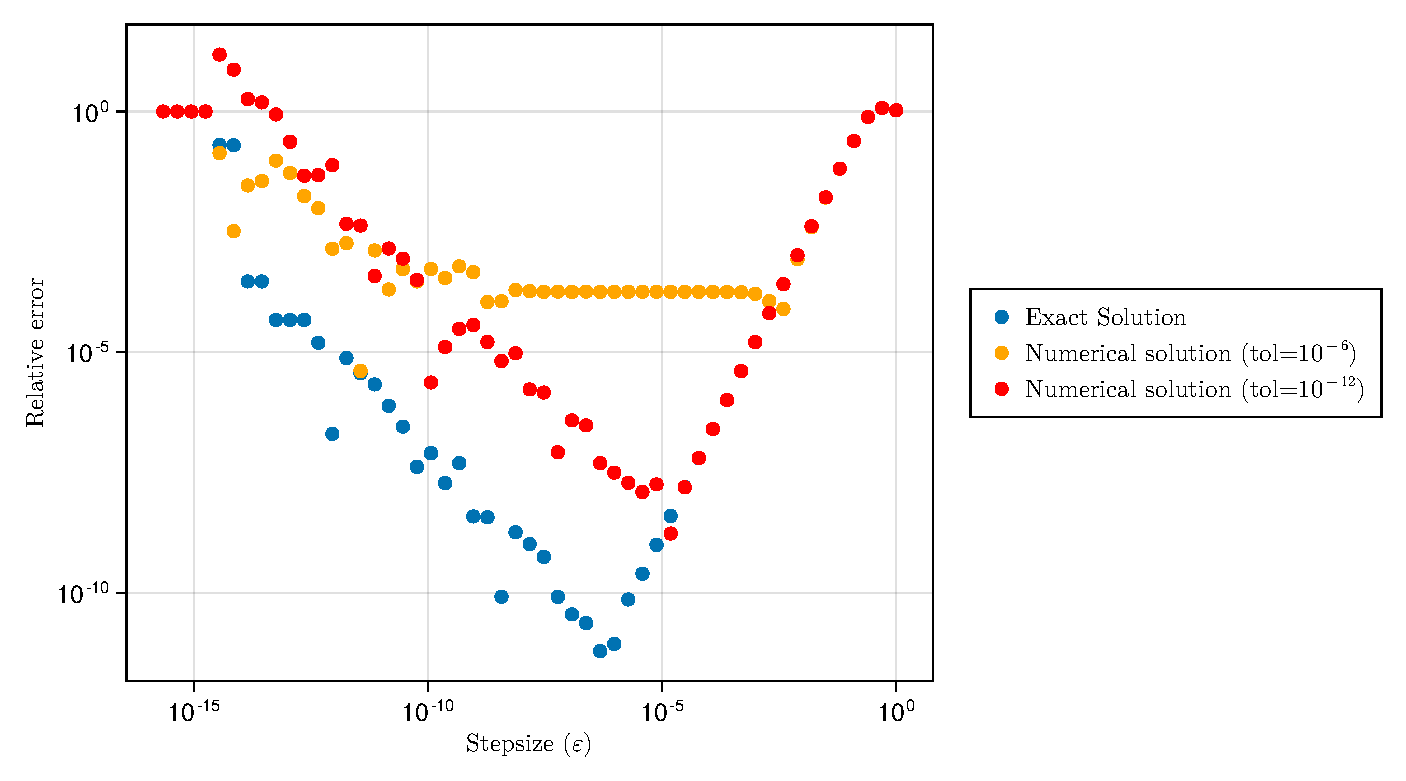
\includegraphics[width=0.85\textwidth]{../code/finite_differences/finite_difference_derivative.pdf}
    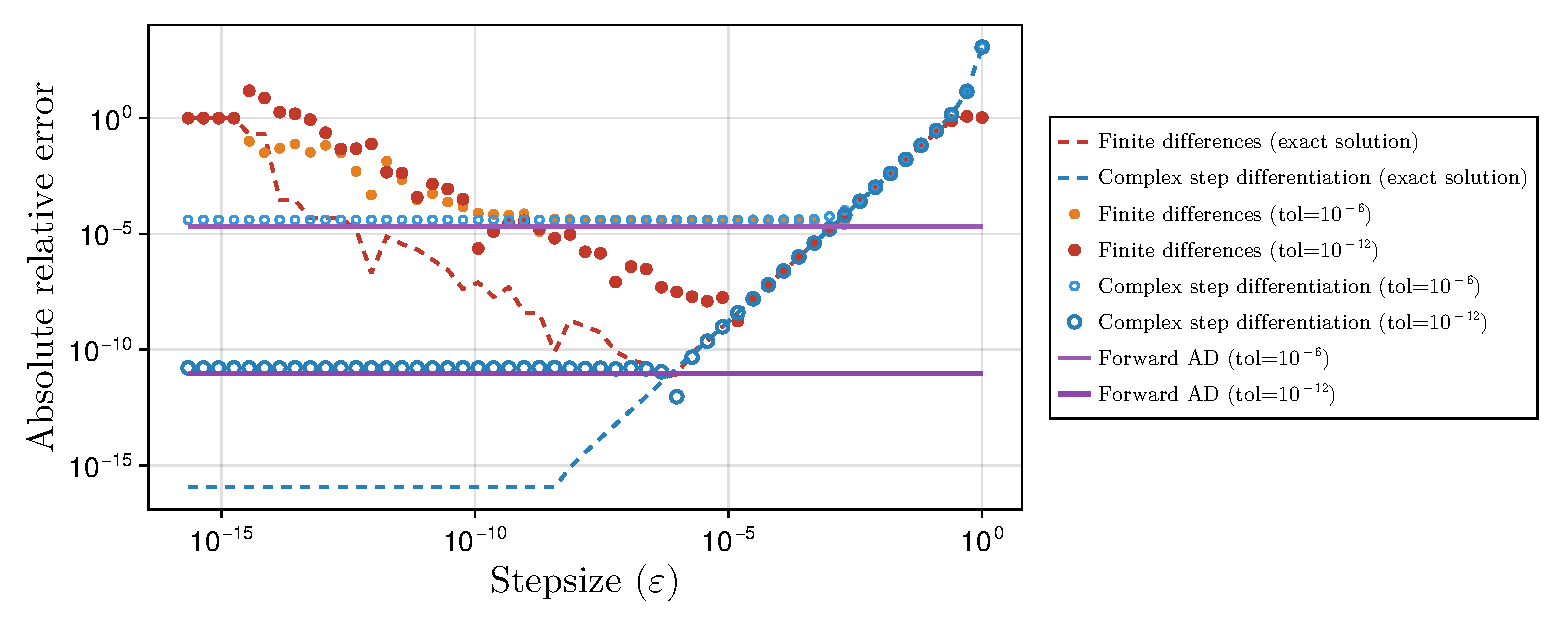
\includegraphics[width=1.0\textwidth]{figures/direct_derivatives.pdf}
    \caption{Absolute relative error when computing the gradient of the function $u(t) = \sin (\theta t)/\theta$ with respect to $\theta$ at $t=10.0$ as a function of the stepsize $\varepsilon$. Here, $u(t)$ corresponds to the solution of the differential equation $u'' + \theta^2 u = 0$ with initial condition $u(0)=0$ and $u'(0)=1$. The blue dots correspond to the case where the relative error is computed with finite differences. The red and orange lines are for the case where $u(t)$ is numerically computed using the default Tsitouras solver \cite{Tsitouras_2011} from \texttt{OrdinaryDiffEq.jl} using different tolerances. The error when using a numerical solver is larger and it is dependent on the numerical precision of the numerical solver. $\clubsuit_\text{\code{code:figure-comparison}}$}
    \label{fig:direct-methods}
\end{figure}

\subsubsection{Automatic differentiation}

The AD algorithms described in Section \ref{section:automatic-differentiation} can be implemented using different strategies, namely operator overloading for AD based on dual numbers, and source code transformation for both forward and reverse AD based on the computational graph \cite{martins2001connection}.
In Section \ref{section:software-Forward-AD} we first cover how forward AD is implemented using dual numbers, postponing the discussion about the implementation using computational graphs for reverse AD in Section \ref{sec:software-reverse-AD}. 

\paragraph{Forward AD based on dual numbers}
\label{section:software-Forward-AD}

Implementing forward AD using dual numbers is usually carried out using operator overloading \cite{Neuenhofen_2018}. 
This means expanding the object associated with a numerical value to include the tangent and extending the definition of atomic algebraic functions. 
In Julia, this can be done by relying on multiple dispatch \cite{Julialang_2017}. 
The following example illustrates how to define a dual number and its associated binary addition and multiplication extensions $\clubsuit_\text{\code{code:dual-number}}$. 
\begin{jllisting}
@kwdef struct DualNumber{F <: AbstractFloat}
    value::F
    derivative::F
end

# Binary sum
Base.:(+)(a::DualNumber, b::DualNumber) = DualNumber(value = a.value + b.value, derivative = a.derivative + b.derivative)

# Binary product 
Base.:(*)(a::DualNumber, b::DualNumber) = DualNumber(value = a.value * b.value, derivative = a.value*b.derivative + a.derivative*b.value)
\end{jllisting}
We further overload base operations for this new type to extend the definition of standard functions by simply applying the chain rule and storing the derivative in the dual variable following Equation \eqref{eq:dual-number-function}:
\begin{jllisting}
function Base.:(sin)(a::DualNumber)
    value = sin(a.value)
    derivative = a.derivative * cos(a.value)
    return DualNumber(value=value, derivative=derivative)
end
\end{jllisting}
% With all these pieces together, we are able to propagate forward the value of a single-valued derivative through a series of algebraic operations. 

In the Julia ecosystem, \texttt{ForwardDiff.jl} implements forward mode AD with multidimensional dual numbers \cite{RevelsLubinPapamarkou2016}. 
% and the sensitivity method \texttt{ForwardDiffSensitivity} implements forward differentiation inside the numerical solver using dual numbers. 
While \texttt{ForwardDiff.jl} defines the interface for defining the tangent of primitive operations, the tangent of different operations are implemented in \texttt{DiffRules.jl}. 
Figure \ref{fig:direct-methods} shows the result of performing forward AD inside the numerical solver.
We can see that for this simple example forward AD performs as good as the best output of finite differences and complex step differentiation (see Section \ref{section:software-complex-step}) when optimizing by the stepsize $\varepsilon$. 
% Further notice that AD is not subject to same level of numerical errors due to floating point arithmetic \cite{Griewank:2008kh}.
% \begin{jllisting}
% using OrdinaryDiffEq, ForwardDiff, Test 
% s_AD = ForwardDiff.jacobian(p -> solve(ODEProblem(f, u0, tspan, p), Tsit5()).u[end], p)
% \end{jllisting}
Implementations of forward AD using dual numbers and computational graphs require a number of operations that increases with the number of variables to differentiate, since each computed quantity is accompanied by the corresponding derivative calculations \cite{Griewank_1989}. 
This consideration also applies to the other forward methods, including finite differences and complex-step differentiation.

\paragraph{Reverse AD based on computational graph}
\label{sec:software-reverse-AD}

In contrast to finite differences, forward AD, and complex-step differentiation, reverse AD is the only of this family of methods that propagates the gradient in reverse mode by relying on analytical derivatives of primitive functions.
The interface for defining primitives in implemented in \texttt{ChainRulesCore.jl}, while the primitives themselves are defined in different libraries (eg, \texttt{ChainRules.jl}, \texttt{SciMLSenstivity.jl}, \texttt{NNlib.jl}). 
% Since reverse AD requires the evaluation of intermediate variables, reverse AD requires a more delicate protocol of how to store intermediate variables in memory and make them accessible during the backwards pass. 
Reverse AD can be implemented via pullback functions \cite{Innes_2018}, a method also known as continuation-passing style \cite{Wang_Zheng_Decker_Wu_Essertel_Rompf_2019}.
In the backward step, it executes a series of function calls, one for each elementary operation.
If one of the nodes in the graph $w$ is the output of an operation involving the nodes $v_1, \ldots, v_m$, where $v_i \rightarrow w$ are all edges in the graph, then the pullback $\bar v_1, \ldots, \bar v_m = \mathcal B_w(\bar w)$ is a function that accepts gradients with respect to $w$ (defined as $\bar w$) and returns gradients with respect to each $v_i$ (defined as $\bar v_i$) by applying the chain rule. 
Consider the example of the multiplication $w = v_1 \cdot v_2$. 
Then
\begin{equation}
 \bar v_1, \, \bar v_2 
 \,=\,
 v_2 \cdot \bar w , \,
 v_1 \cdot \bar w 
 \,=\,
 \mathcal{B}_w (\bar w),
\end{equation}
which is equivalent to using the chain rule as
\begin{equation}
 \frac{\partial \ell}{\partial v_1} 
 = \frac{\partial}{\partial v_1}(v_1 \cdot v_2) \frac{\partial \ell}{\partial w}
 =
 v_2 \cdot \bar w \, , \qquad 
 \frac{\partial \ell}{\partial v_2} = v_1 \cdot \bar \omega \, .
\end{equation}

A crucial distinction between AD implementations based on computational graphs is between \textit{static} and \textit{dynamic} methods \cite{Baydin_Pearlmutter_Radul_Siskind_2015}. 
In the case of a static implementations, the computational graph is constructed before any code is executed, which are encoded and optimized for performance within the graph language. 
For static structures such as neural networks, this is ideal, as it simplifies performance optimizations to be applied \cite{abadi-tensorflow}. 
However, two major drawbacks of static methods are composability with existing code, including support of custom types, and adaptive control flow, which is a common feature of numerical solvers. 
In the case of dynamic methods, these issues are addressed using \textit{tracing} or tape-based implementations, where the program structure is transformed into a list of pullback functions that build the graph dynamically at runtime. 
Popular Julia libraries falling in this category are \texttt{Tracker.jl} and \texttt{ReverseDiff.jl}. 
A major drawback of tracing systems is that the pullbacks are constructed with respect to the control flow of the input value and thus do not necessarily generalize to other inputs. 
This means that the pullback must be reconstructed for each forward pass, limiting the reuse of computational optimizations and inducing higher overhead. 
Source-to-source AD systems can achieve higher performance by giving a static derivative representation to arbitrary control flow structure, thus allowing for the construction and optimization of pullbacks independent of the input value. 
These include \texttt{Zygote.jl} \cite{Innes_Zygote}, \texttt{Enzyme.jl} \cite{moses_Enzyme, Moses.2021}, and \texttt{Diffractor.jl}.
The existence of these multiple AD packages lead to the development of \texttt{AbstractDifferentiation.jl} which allows one to combine different methods \cite{Schäfer_Tarek_White_Rackauckas_2021}. 

% It is important to mention that incorrect implementations of both forward and reverse AD can lead to \textit{perturbation confusion}, an existing problem in some AD software where either repeated applications of AD or differentiation with respect to different dual variables result indistinguishable \cite{siskind2005perturbation, manzyuk2019perturbation}. 

\paragraph{Discrete checkpointing}
\label{section:checkpointing}

In contrast to forward methods, all reverse methods, including backpropagation and adjoint methods, require to access the value of intermediate variables during the propagation of the gradient. 
For a numerical solver or for time-stepping codes, the number of memory required to accomplish this can be very large, involving a total of at least $\mathcal O(nk)$ terms, with $k$ the number of steps of the numerical solver (or the number of time steps). 
Checkpointing is a technique that can be used for all reverse methods. 
It avoids storing all the intermediate states by balancing  storing and recomputation to recover the required state exactly \cite{Griewank:2008kh}.
This is achieved by saving intermediate states of the solution in the forward pass and recalculating the solution between intermediate states in the reverse mode. 
Different checkpointing algorithms have been proposed, ranging from static or uniform, multi-level \cite{Giering_Kaminski_1998,Heimbach.2005} to optimized, binomial checkpointing algorithms  \cite{Griewank.2000,Walther.2004,Bockhorn.2020,Checkpoiting_2023}.

% Talk about MALI \cite{Zhuang_Dvornek_Tatikonda_Duncan_2021}. 
% Margossian has a nice discussion on this topic

\paragraph{When AD is algorithmically correct but numerically wrong}
\label{section:AD-incorrect}


% In this section, we are going to consider certain errors that can potentially show up when combining AD with a numerical solver. 
Although AD is always algorithmically correct, when combined with a numerical solver \textit{AD can be numerically incorrect} and result in wrong gradient calculations \cite{Eberhard_Bischof_1996}. 
In this section we are going to show an example where AD fails when directly applied to an unmodified solution computed with an adaptive stepsize numerical solver (see Section \ref{section:intro-numerical-solvers}).
% As explained in Section \ref{section:intro-numerical-solvers}, traditional adaptive stepsize solvers used for just solving ODEs are designed to control for numerical errors in the ODE solution. 
When performing forward AD though numerical solver, the error used in the stepsize controller needs to naturally account for both the errors induced in the numerical solution of the original ODE and the errors in the dual component carrying the value of the sensitivity. 
This relation between the numerical solver and AD has been made explicit when we presented the relationship between forward AD and the forward sensitivity equations (Section \ref{section:forwardAD-sensitivity}). 

To illustrate this, let us consider the following first-order ODE:
\begin{equation}
\begin{cases}
 \frac{du_1}{dt} = a u_1 - u_1 u_2 & \quad u_1(0) = 1  \\ 
 \frac{du_2}{dt} = - a u_2 + u_1 u_2 & \quad u_2(0) = 1.
\end{cases}
\end{equation}
Notice that for the value of the parameter $a = 1$, this ODE admits an analytical solution $u_1(t) \equiv u_2(t) \equiv 1$, making this problem very simple to solve numerically.
The following code solves for the derivative with respect to the parameter $a$ using two different methods. 
The second method using forward AD with dual numbers declares the \texttt{internalnorm} argument according to Equation \eqref{eq:internal-norm-wrong} $\clubsuit_\text{\code{code:AD-wrong}}$.
\begin{jllisting}
using SciMLSensitivity, OrdinaryDiffEq, Zygote, ForwardDiff

function fiip(du, u, p, t)
    du[1] =  p[1] * u[1] - u[1] * u[2]
    du[2] = -p[1] * u[2] + u[1] * u[2]
end

p = [1.]
u0 = [1.0;1.0]
prob = ODEProblem(fiip, u0, (0.0, 10.0), p);

# Correct gradient computed using 
grad0 = Zygote.gradient(p->sum(solve(prob, Tsit5(), u0=u0, p=p, sensealg = ForwardSensitivity(), saveat = 0.1, abstol=1e-12, reltol=1e-12)), p)
# grad0 = ([212.71042521681443],)

# Original AD with wrong norm 
grad1 = Zygote.gradient(p->sum(solve(prob, Tsit5(), u0=u0, p=p, sensealg = ForwardDiffSensitivity(), saveat = 0.1, internalnorm = (u,t) -> sum(abs2,u/length(u)), abstol=1e-12, reltol=1e-12)), p)
# grad1 = ([6278.15677493293],)
\end{jllisting}
The reason why the two methods give different answers is because the error estimation by the stepsize controller is ignoring numerical errors in the dual component. 
In the later case, since the numerical solution of the original ODE is constant, the local estimated error is drastically underestimated to $\text{err}_i^{m} = 0$, which makes the stepsize $\Delta t_{m}$ to increase by a multiplicative factor at every step (see Equations \eqref{eq:internal-norm-wrong} and \eqref{eq:PIC}). 
This can be fixed by instead considering a norm that accounts for both the primal and dual components in the forward pass, 
\begin{align}
    \text{Err}_\text{scaled}^{m}
    =
    \Bigg [ \frac{1}{n(p+1)} \Bigg( 
    &\sum_{i=1}^n \left( \frac{u_i^{m} - \hat u_i^{m}}{\mathfrak{abstol} + \mathfrak{reltol} \times \max \{ u_i^{m}, \hat u_i^{m}\}} \right)^2 \nonumber \\
    + 
    &\sum_{i=1}^n \sum_{j=1}^p  
    \left( \frac{s_{ij}^{m} - \hat s_{ij}^{m}}{\mathfrak{abstol} + \mathfrak{reltol} \times \max \{ s_{ij}^{m}, \hat s_{ij}^{m}\}} \Bigg)^2 \right)
    \Bigg ]^{\frac{1}{2}},
    \label{eq:internal-norm-correct} 
\end{align}
with $s^m$ and $\hat s^m$ two different numerical approximations of the sensitivity matrix. 
This correction now gives the right answer:
\begin{jllisting}
sse(x::Number) = x^2
sse(x::ForwardDiff.Dual) = sse(ForwardDiff.value(x)) + sum(sse, ForwardDiff.partials(x))

totallength(x::Number) = 1
totallength(x::ForwardDiff.Dual) = totallength(ForwardDiff.value(x)) + sum(totallength, ForwardDiff.partials(x))
totallength(x::AbstractArray) = sum(totallength,x)

grad3 = Zygote.gradient(p->sum(solve(prob, Tsit5(), u0=u0, p=p, sensealg = ForwardDiffSensitivity(), saveat = 0.1, internalnorm = (u,t) -> sqrt(sum(x->sse(x),u) / totallength(u)), abstol=abstol, reltol=reltol)), p)
# grad3 = ([212.71042521681392],)
\end{jllisting}
This is an example where the form of the numerical solver for the original ODE is affected by the fact we are simultaneously solving for the sensitivity. 
Notice that current implementations of forward AD inside \texttt{SciMLSensitivity.jl} already accounts for this and there is no need to specify the internal norm $\clubsuit_\text{\ref{code:AD-wrong}}$. 
To highlight the pervasiveness of this issue with respect to AD, we further provide a script with an example in \texttt{Diffrax} where the derivative that does not converge to the correct answer as tolerance is decreased to zero $\clubsuit_\text{\code{code:AD-wrong-JAX}}$.

\paragraph{Differentiation with sparsity}
\label{section:sparsity}

The total number of computations required to evaluate a gradient/Jacobian using any direct method will depend of its sparsity.  
When the sparsity pattern is known, colored AD efficiently chunk the calculation of the Jacobian into multiple JVPs or VJPs \cite{gebremedhin2005color}. 
This results in a smaller number of evaluations of VJPs/JVPs compared to the one required to compute all entries of a dense Jacobian \cite{pal2024nonlinearsolve}. 
This can represent a significant advantage for large-scale nonlinear systems and discretized PDEs where sparse Jacobian are commonplace.  

Generally AD is recommended as a direct differentiation method due to its generality on programs and the lack of potential memory issues by avoiding expression swell, though there are some situations where symbolic differentiation may be appropriate. 
For example, there are certain sparsity patterns by which even colored AD  requires computing the full Jacobian via all columns/rows, while computing the sparse Jacobian element-by-element using symbolic differentiation only requires computing the non-zero elements.
In other words, depending  of the sparsity pattern, symbolic differentiation can be more efficient than AD \cite{Lantoine_Russell_Dargent_2012}.
% In Section \ref{sec:vjp-jvp} we discussed how colored AD can be used to efficiently compute a sparse Jacobian.
% This is because colored AD has the limitation that an extremely sparse matrix can have no rows or columns independent of each other. 
An example of this is given by the arrowhead matrix $J_{\text{arrowhead}} \in \R^{n \times n}$ given by:
\begin{equation}
    J_{\text{arrowhead}} = \begin{bmatrix}
        \bullet & \bullet & \bullet & \bullet & \cdots & \bullet  & \bullet   \\
        \bullet & \bullet & 0  &  0    &   & 0        & 0        \\
        \bullet & 0 & \bullet & 0 & & 0        & 0        \\
        \bullet & 0 & 0 & \bullet & & 0 & 0 \\
        \vdots & & & & \ddots & &  \\
        \bullet & 0 & 0 & 0   &   & \bullet   & 0        \\
        \bullet & 0 & 0        & 0    &    & 0        & \bullet
    \end{bmatrix},
\end{equation}
where $\bullet$ indicate non trivial zero entries of the Jacobian.
In this case, both forward and reverse AD will have to perform $n$ VJPs and JVPs, respectively, and there is no computational benefit of using colored AD. 
Instead, symbolic differentiation constructs a symbolic representation of the sparse Jacobian entry-by-entry and can fill the Jacobian with $n + 2 \cdot (n-1)$ computations, where each computation is significantly cheaper than each VJP or JVP. 
Notice that for the arrowhead matrix example, a combination of forward and reverse AD can be used to color the Jacobian with two forward and one reverse AD evaluation. 
% This may be worth adding, but not sure yet.
% Consider the example given in \cite{Griewank:2008kh}
% \begin{equation}
%     L(x) = \ln \Psi_0 = \ln \sum_{i=1}^d w_i \Psi_i (e^{z_i \sin (x)}) 
% \end{equation}
% with $0 \geq w_i$ and $z_i \in \R$ some coefficients and $\Psi_i : \R \mapsto \R_{\geq 0}$. 
% Computer algebra systems are able to handle the common sub-expression $\cos(x) / \Psi_0 $ in $L'(x)$ to reduce the total number of multiplication involved in the derivative with respect to both forward and reverse AD, which instead will evaluate the sub-product with respect to the term   $\cos(x) / \Psi_0$.

% Talk about unmodified solutions..


\subsubsection{Complex step differentiation}
\label{section:software-complex-step}
% For credit: The figure in the left coicindes with the one in  \cite{fike2013multi}
% Read more carefully Martins et. al. (2001) for the computational aspects of complex step.

Modern software already have support for complex number arithmetic, making complex step differentiation very easy to implement.
In Julia, complex analysis arithmetic can be easily carried inside the numerical solver.
The following example shows how to extend the numerical solver used to solve the ODE in Equation \eqref{eq:example-ode-direct-methods} to support complex numbers $\clubsuit_\text{\code{code:complex-step}}$.
\begin{jllisting}
function dyn!(du::Array{Complex{Float64}}, u::Array{Complex{Float64}}, p, t)
    ω = p[1]
    du[1] = u[2]
    du[2] = - ω^2 * u[1]
end

tspan = [0.0, 10.0]
du = Array{Complex{Float64}}([0.0])
u0 = Array{Complex{Float64}}([0.0, 1.0])

function complexstep_differentiation(f::Function, p::Float64, ε::Float64)
    p_complex = p + ε * im
    return imag(f(p_complex)) / ε
end

complexstep_differentiation(x -> solve(ODEProblem(dyn!, u0, tspan, [x]), Tsit5()).u[end][1], 20., 1e-3)
\end{jllisting}

Figure \ref{fig:direct-methods} further shows the result of performing complex step differentiation using the same example as in Section \ref{section:software-finite-differences}.
We can see from both exact and numerical solution that complex-step differentiation does not suffer from small values of $\varepsilon$, meaning that $\varepsilon$ can be chosen arbitrarily small \cite{martins2001connection} as long as it does not reach the underflow threshold \cite{Goldberg_1991_floatingpoint}. 
Notice that for large values of the stepsize $\varepsilon$ complex step differentiation gives similar results to finite differences, while for small values of $\varepsilon$ the performance of complex step differentiation is slightly worse than AD. 
This result emphasizes the observation made in Section \ref{section:comparison-discrete-adjoint-AD}, namely that complex step differentiation has many aspects in common with finite differences and AD based on dual numbers. 

% This resemblance between the methods makes them susceptible to the same advantages and disadvantages: easiness of implementation with operator overloading; and inefficient scaling with respect to the number of variables to differentiate. 
However, the difference between the methods also makes the complex step differentiation sometimes more efficient than both finite differences and AD \cite{Lantoine_Russell_Dargent_2012}, an effect that can be counterbalanced by the number of extra unnecessary operations that complex arithmetic requires (see last column in Figure \ref{fig:complex-step-AD}) \cite{Martins_Sturdza_Alonso_2003_complex_differentiation}.
Further notice that complex-step differentiation will work as long as every function involved in the computation is locally analytical. 
This is a problem with implementations of functions that rely on the absolute function, for example using complex step differentiation on the square function implemented as $f(z) = \text{abs}(z)^2$ will always return zero ($\text{Im}(f(x + i \varepsilon))= \text{Im}((x + i \epsilon)(x - i \epsilon)) = \mathcal O (\varepsilon^2)$).